\chapter{Comportamento del Sistema}
\section{Descrizione della Rete di Petri}
% Descrizione del comportamento del sistema (ad un certo livello di astrazione)
% utilizzando Reti di Petri.
Il comportamento del sistema è stato modellato, ad un certo livello di astrazione, utilizzando una Rete di Petri.
\begin{question}[Rete di Petri]
Una Rete di Petri è un approccio grafico alla rappresentazione dei sistemi ad eventi in cui è possibile che alcuni eventi occorrano concorrentemente. Si tratta di un modello formale astratto del flusso di informazioni, descrive ed analizza il flusso di informazioni del sistema.
\end{question}
Il flusso di controllo inizia dalla piazza \textit{start}, l'unica transizione attiva è \textit{initialization}, la quale si occupa di creare 8 token che rappresentano i \textit{workers} (ovvero i thread) e 12 token che rappresentano i documenti PDF nel path specificato.
\begin{warn}[NOTA:]
Al fine di astrarre il funzionamento del sistema, si assume per semplicità di utilizzare 8 thread e un numero di file PDF pari a 12. Non è possibile specificare valori generici sul peso degli archi, per cui non è possibile testare esaustivamente tutti gli scenari, anche a causa di quanto computazionalmente sarebbe dispendioso il processo.
\end{warn}
I workers non hanno ancora task da poter elaborare, per cui l'unica transizione attiva è \textit{create file read task}. All'interno di questa transizione avviene il caricamento del file in memoria, in quanto viene creato un \textit{file read task} da aggiungere alla bag of tasks. Questa transizione, (\textit{create file read task}) rimane attiva finché ci saranno ancora token nella piazza \textit{pdf in path}.\newline
Se esiste almeno un \textit{file read task} ed almeno un \textit{worker} è disponibile, allora la transizione \textit{begin file read task} è attiva, e il task viene eseguito. Il task legge il contenuto del documento e solo una volta che avrà terminato tenterà di acquisire il permesso di entare in sezione critica, poiché deve accedere ad una struttura dati condivisa da tutti gli altri workers.\newline
Il meccanismo appena descritto viene rappresentato nella Petri Net dalla transizione \textit{acquire final map lock}.\newline
La transizione \textit{acquire final map lock} però è attiva solo qualora sia disponibile un token all'interno della piazza \textit{final map token}. Se il token non è presente significa che un altro worker si trova all'interno della sezione critica, e quindi la transizione non sarà abilitata finché quest'ultimo non avrà terminato di aggiornare la struttura dati condivisa.\newline
Una volta terminato l'aggiornamento della struttra dati è possibile per altri worker acquisire il permesso di entrare in sezione critica, e il worker tornerà disponibile per eseguire un nuovo task.\newline
La rete di Petri appena presentata è bounded e termina sempre.\newline
Nello stato finale della Petri Net ci sarà un numero di token pari a 8 nella piazza \textit{workers} e un token nella piazza \textit{final map token}.
\begin{info}
Una Rete di Petri è bounded solo se ha un numero finito di stati possibili.
\end{info}
\begin{figure}[H]
	\begin{center}
		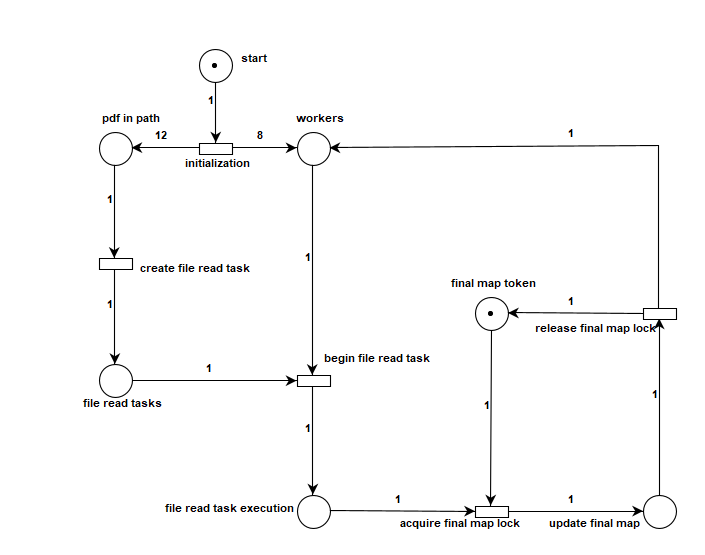
\includegraphics[width=\linewidth]{img/petrinet.png}
		\label{fig:petrinet}
		\caption{Rete di Petri del sistema}
	\end{center}
\end{figure}
